\begin{landscape}
	\subsubsection{Poziom 1}
		\begin{figure}[H]
			\centering
			\centerline{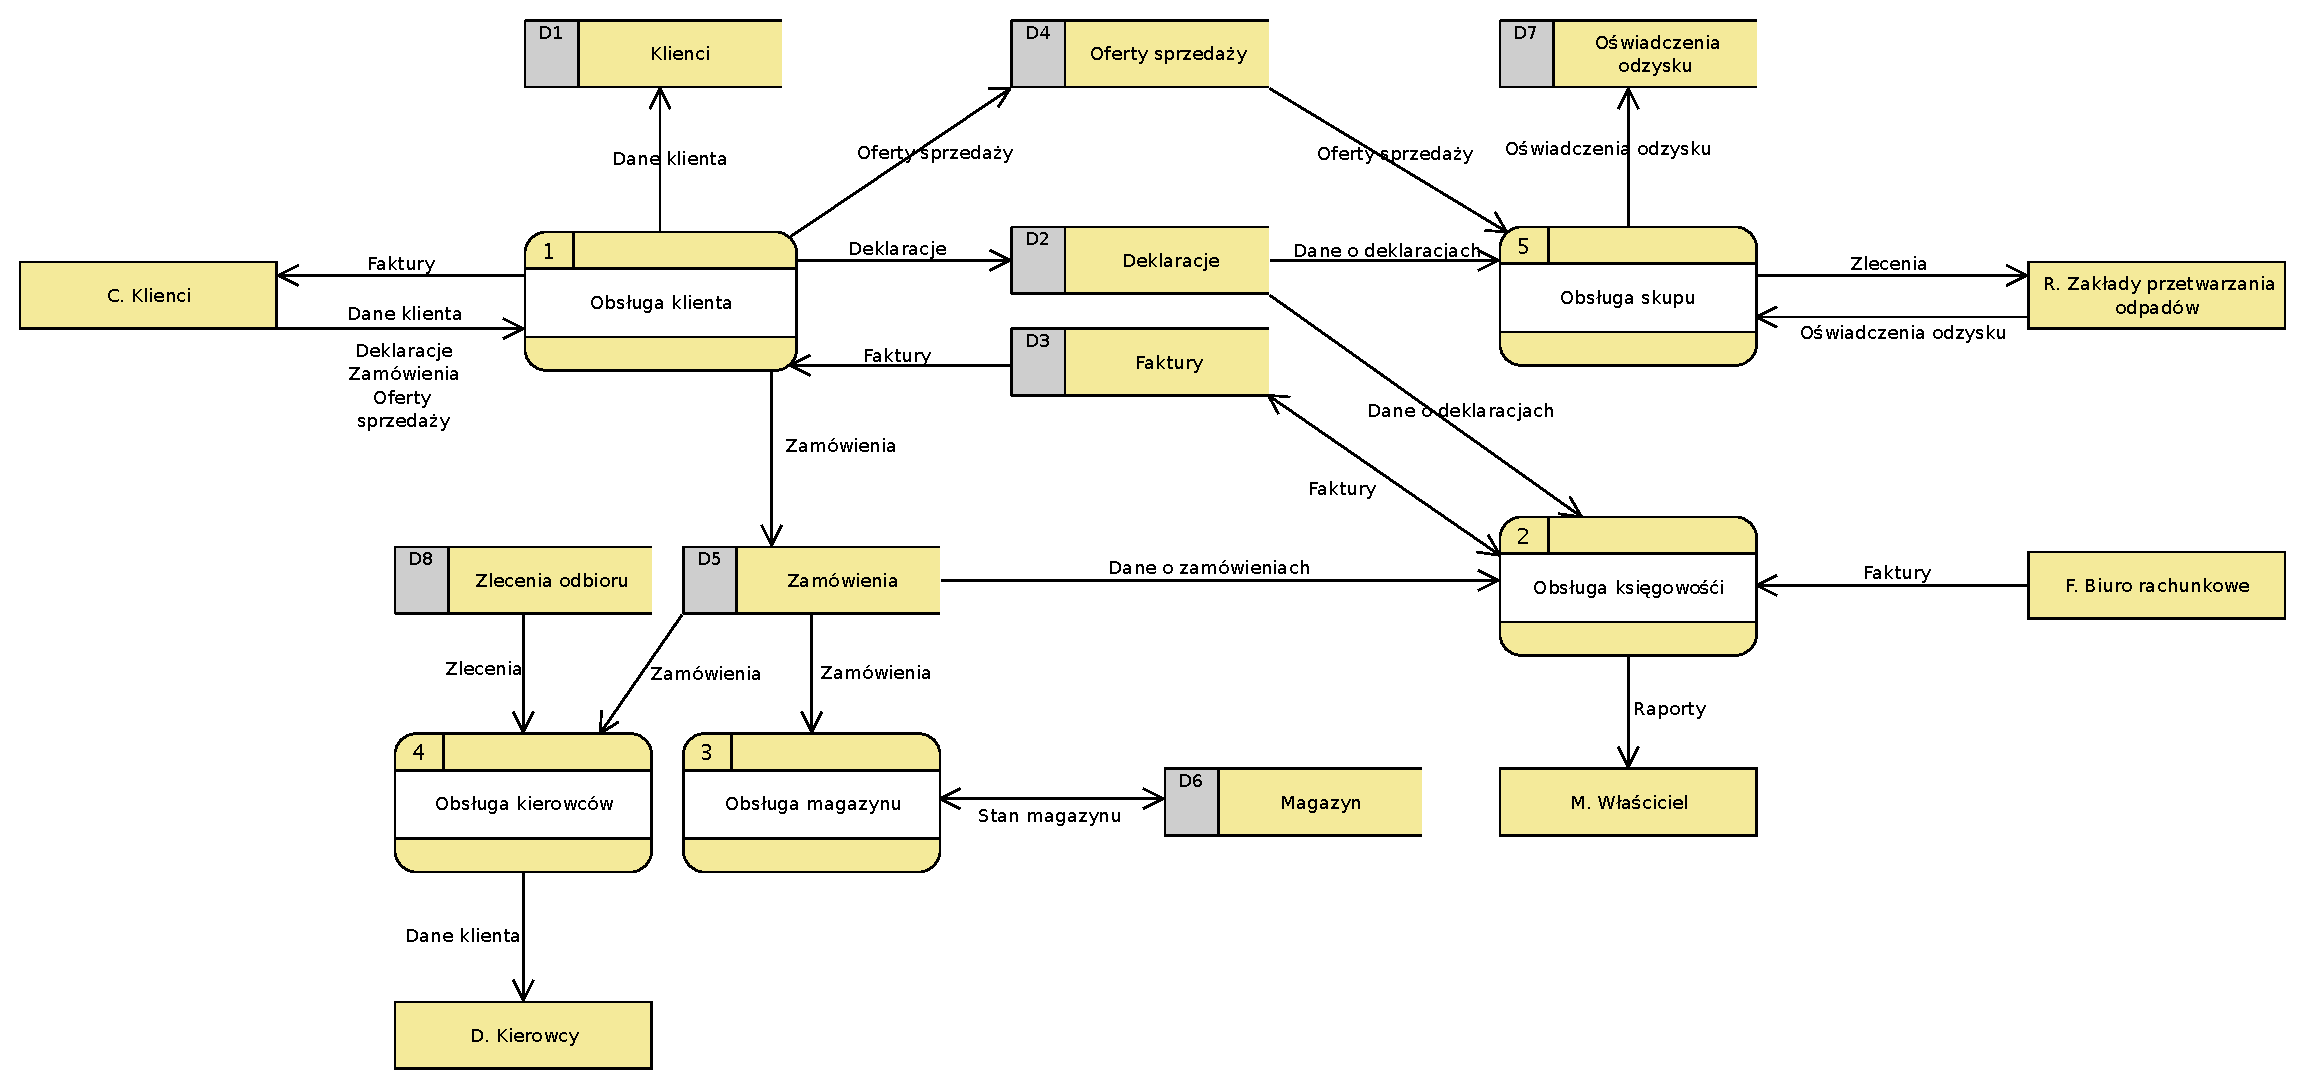
\includegraphics[width=29cm]{img/DFD/1-level.eps}}
		\end{figure}
\end{landscape}

	%DFD1
	\textbf{Opis}\\
	Digram pokazuje wyodrębnienie podsystemów, które są przedstawione bardziej szczegółowo na kolejnych diagramach.\\
	Część funckjonalności dotyczącej wspomagania pracy właściciela realizowana jest w podsystemie \textbf{3. Obsługa księgowości}.

	

\subsubsection{Poziom 2}

	\begin{figure}[H]
		\centering
		\centerline{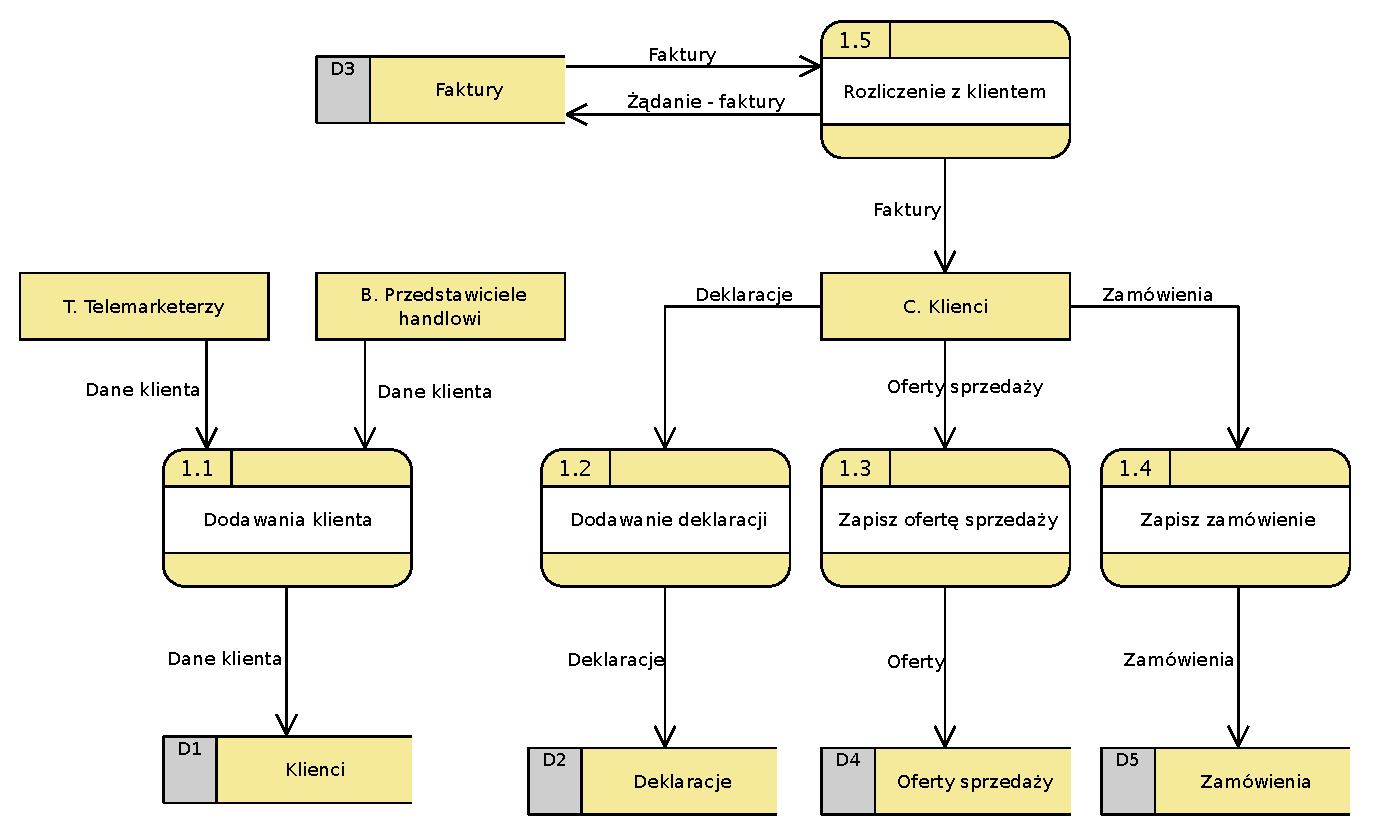
\includegraphics[width=1.2\textwidth]{img/DFD/2-level-klient.eps}}
		\caption{Obsługa klienta}
	\end{figure}

	\begin{figure}[H]
		\centering
		\centerline{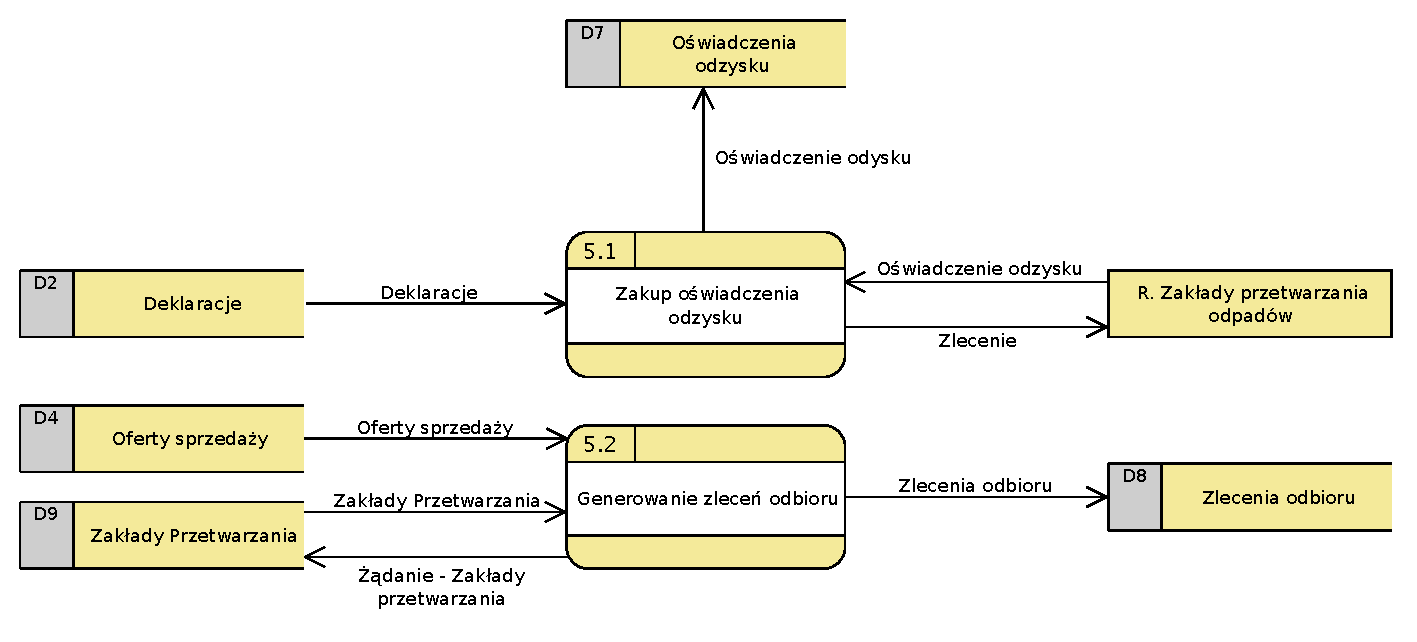
\includegraphics[width=1.1\textwidth]{img/DFD/2-level-skup.eps}}
		\caption{Obsługa skupu}
	\end{figure}
	
	\textbf{Opis} \\
	\underline{2.1 Zakup oświadczenia odzysku}\\
	Pracownik działu skupu kupuje oświadczenie odzysku na podstawie deklaracji, aby wprowadzić je do bazy \\
	\textbf{Strumień wejściowy} Deklaracja \\
	\textbf{Strumień wyjściowy} Oświadczenie Skupu \\
	
	\underline{2.2 Generowanie zleceń odbioru}\\
	Generowanie zlecenia odbioru na podstawie Ofert Sprzedaży w celu przydzielenia kierowcy
	\textbf{Strumień wejściowy} Oferta sprzedaży \\
	\textbf{Strumień wyjściowy} Zlecenie odbioru, Żądanie \\
	
	\begin{figure}[H]
		\centering
		\centerline{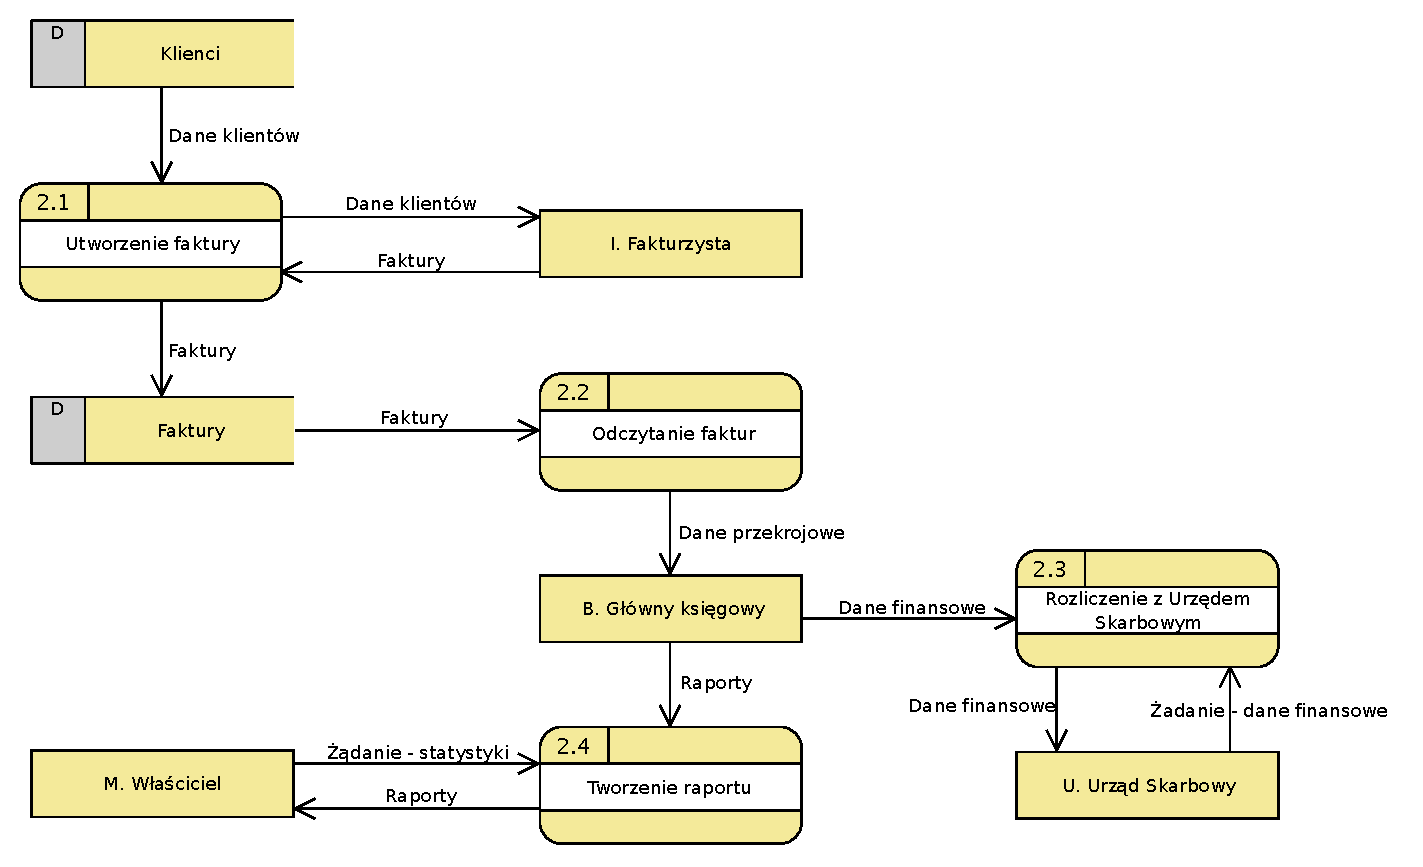
\includegraphics[width=1.1\textwidth]{img/DFD/2-level-ksiegowosc.eps}}
		\caption{Obsługa księgowości}
	\end{figure}

	\begin{figure}[H]
		\centering
		\centerline{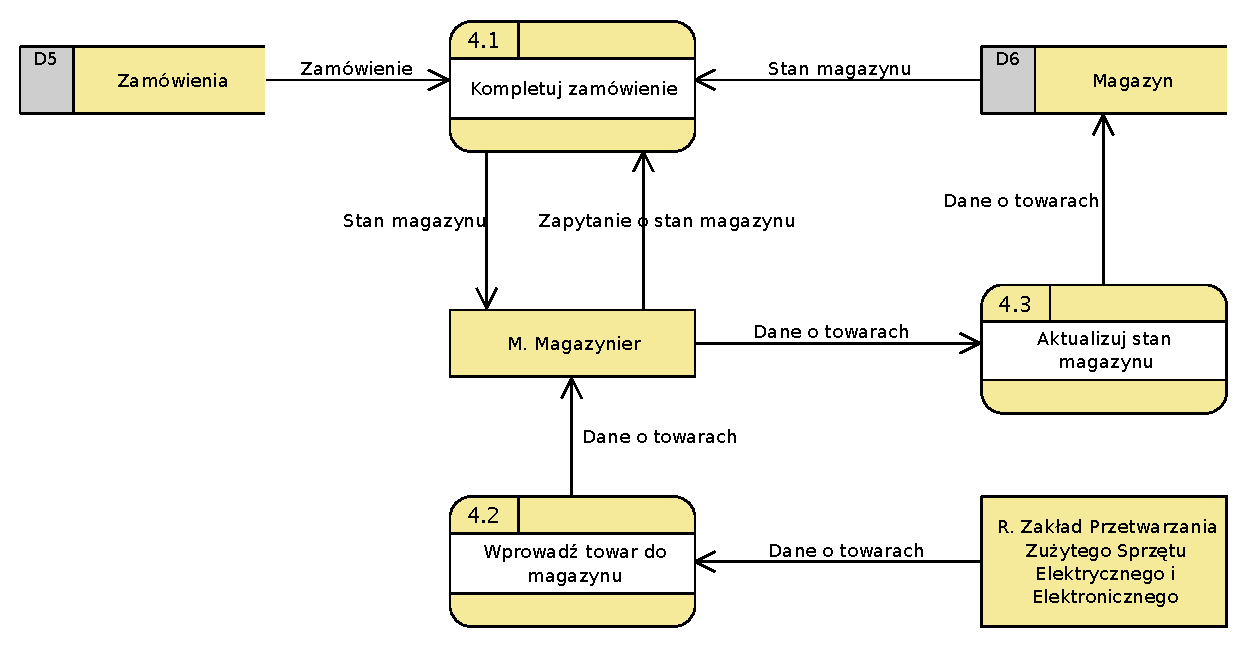
\includegraphics[width=1.1\textwidth]{img/DFD/2-level-magazyn.eps}}
		\caption{Obsługa magazynu}
	\end{figure}

	\textbf{Opis} \\
	\underline{4.1 Kompletuj zamówienie}\\
	Magazynier pyta o stan magazynu, aby sprawdzić, czy może skompletować zamówienie.
	\textbf{Strumień wejściowy} zapytanie o stan magazynu, zamówienie\\
	\textbf{Strumień wyjściowy} aktualny stan magazynu\\

	\underline{4.2 Aktualizuj stan magazynu}\\ 
	Stan magazynu jest aktualizowany na podstawie ilości produktów dostarczanych lub odbieranych.\\	
	\textbf{Strumień wejściowy} Produkty przyjmawane do magazynu, produkty wydawane przez magazyn.\\
	\textbf{Strumień wyjściowy} Produkty przyjmawane do magazynu, produkty wydawane przez magazyn.\\
	
	\underline{4.3 Wprowadź towar do magazynu}\\
	Towar zostaje przywieziony przez kierowcę z Zakładu Przetwarzania Zużytego Sprzętu Elektrycznego i Elektronicznego, informacje o jego ilości są zapisywane do systemu.\\
	\textbf{Strumień wejściowy} Dane o przywiezionych towarach\\
	\textbf{Strumień wyjściowy} Dane o przywiezionych towarach\\

	\begin{figure}[H]
		\centering
		\centerline{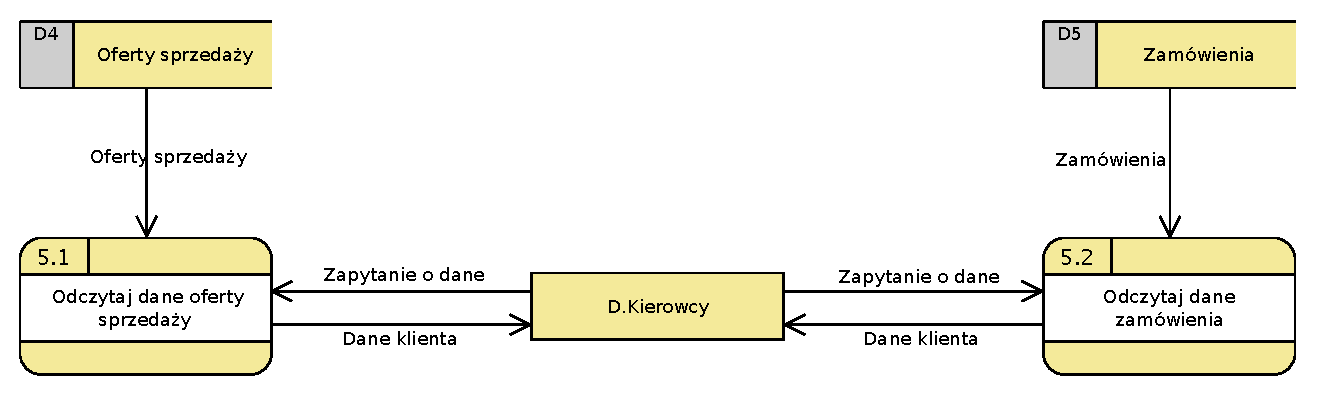
\includegraphics[width=1.1\textwidth]{img/DFD/2-level-kierowcy.eps}}
		\caption{Obsługa kierowców}
	\end{figure}
	
	\textbf{Opis} \\
	\underline{5.1 Odczytaj dane oferty sprzedaży i 5.2 Odczytaj dane zamówienia}\\
	Kierowca pyta o dane klienta, który złożył, odpowiednio Oferte Sprzedaży i Zamówienie\\
	\textbf{Strumień wejściowy} Dane klienta\\